\scanpage{25}
\mspage{8)}
ou encore par un relèvement
\[
(14)\quad\diagram{\begin{tikzcd}
\mathcal M_{X,x}\arrow[r,no head]&\Gamma_{\widetilde{\mathbb Q}/\mathbb Q}\\
&\Gamma_{\overline K/K}\arrow[u]\arrow[ul,dashed]
\end{tikzcd}}
\]
et de même pour $\xi$, correspondant à une restriction du corps de définition
$k$ de $X$ à $K$, ceci correspond à
\[
(14')\quad\diagram{\begin{tikzcd}
\mathcal N_{X,x}\arrow[r,two heads]&\Gamma_{\widetilde{\mathbb Q}/\mathbb Q}\\
&\Gamma_{\overline K/K}\arrow[u]\arrow[ul,dashed]
\end{tikzcd}}
\]
\deleted{\unsure{La donnée donc, puisque}}

\margin{\figure{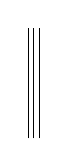
\begin{tikzpicture}\draw (0,0)--(0,1.4);\draw (.07,0)--(.07,1.4);\draw (.14,0)--(.14,1.4);\end{tikzpicture}}}
Je pense que ces données permettent de réconstituer $(K,\overline K,(X,x))$
resp $(K,\overline K,X)$.

J'ai envie d'exprimer la structure de façon plus simple, en notant que (14)
\inserted{resp $(14')$} implique
\[
(15)\qquad\Gamma_{\overline K/K}\longrightarrow\operatorname{Aut}_{\mathrm{loc}}\Pi_{X,x}
\qquad\text{resp.}
\]
\[
(15')\qquad\Gamma_{\overline K/K}\mathbin{-}\operatorname{Autext}_{\mathrm{loc}}(\Pi_{X,x})
\]
\mspage{24}
